
% -----------------------------------------------------------------------------
\begin{figure}
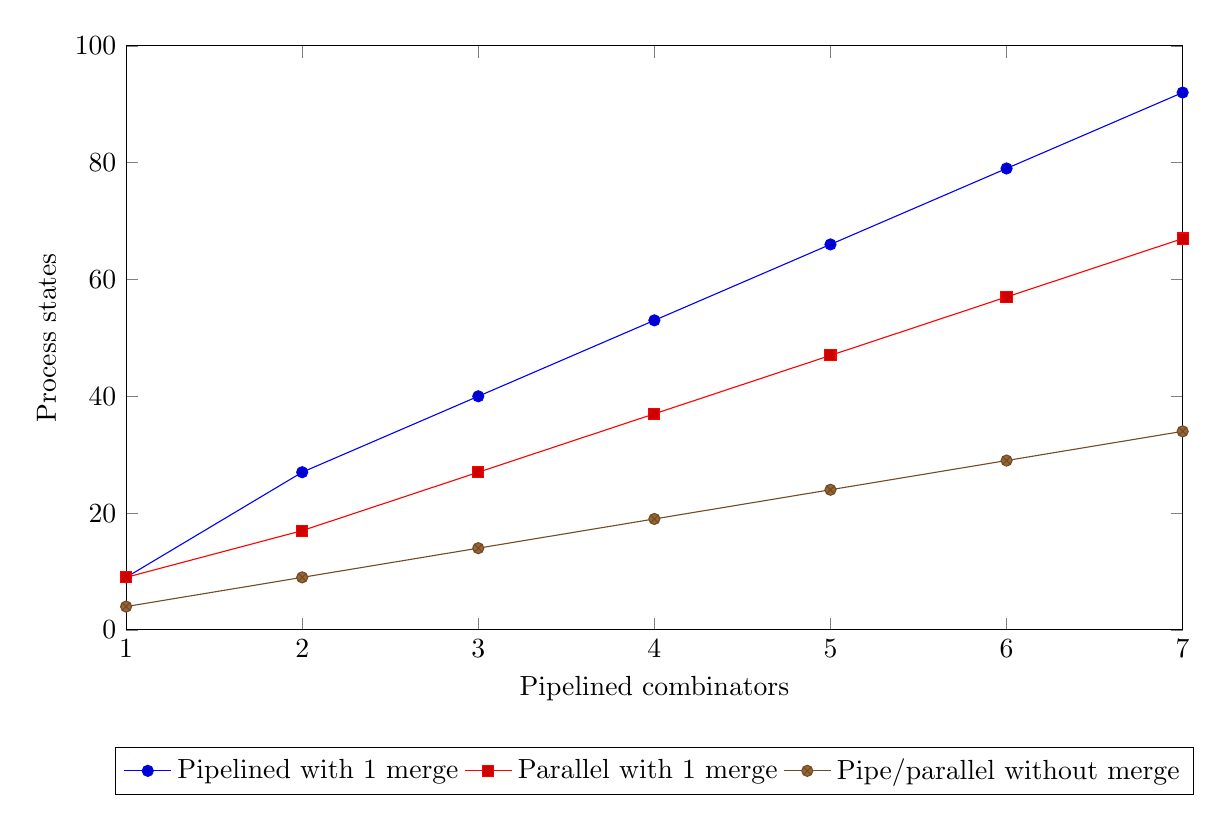
\begin{tikzpicture}
\begin{axis}[
% Hide the label on the second graph
	ylabel=Process states,
	xlabel=Pipelined combinators,
  ymin=0, ymax=100,
  xmin=1, xmax=7,
  xtick=data,
    width=15cm, height=9.0cm,
    legend style={at={(0.5,-0.2)},anchor=north, legend columns=4},
]
\addplot coordinates {(1,9) (2,27) (3,40) (4,53) (5,66) (6,79) (7,92) };
\addplot coordinates {(1,9) (2,17) (3,27) (4,37) (5,47) (6,57) (7,67) };
\addplot coordinates {(1,4) (2,9) (3,14) (4,19) (5,24) (6,29) (7,34)  };

\legend{Pipelined with 1 merge, Parallel with 1 merge, Pipe/parallel without merge};
\end{axis}
\end{tikzpicture}

\caption{Maximum output process size for fusing all combinations of up to $n$ combinators.}
\label{fig:bench:outputsize}
\end{figure}


% -----------------------------------------------------------------------------
\begin{figure}

\begin{tikzpicture}
\begin{axis}[
	ylabel=Process states,
	xlabel=Number of merges,
%  ymode=log,
  ymin=0, ymax=1500,
	enlargelimits=0.01,
  xtick=data,
  xmin=1, xmax=7,
    width=15cm, height=9.0cm,
	legend pos=north west,
]
% These are the values for splitting.
% They are smaller than the 'chaining', but look much nicer on the linear graph.
\addplot coordinates {(1,9) (2,42) (3,97) (4,196) (5,383) (6,746) (7,1461) (8,2880) };

% These are the values for chaining
% \addplot coordinates {(1,4) (2,48) (3,194) (4,760) (5,2814) (6,10064) (7,1) };

\end{axis}
\end{tikzpicture}

\caption{Exponential blowup occurs when splitting or chaining merges together.}
\label{fig:bench:exponential}
\end{figure}

